\section{Int�grer un poste client}
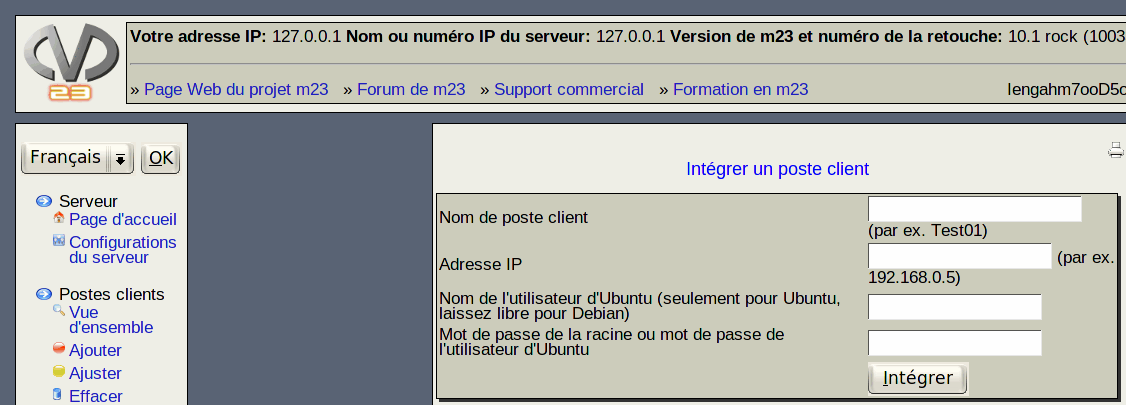
\includegraphics[scale=0.4]{/mdk/doc/manual/screenshots/fr/client_assimilate.png} \\
Vous pouvez administrer des syst\`emes Debian existants avec m23 en les int\'egrant et de cette fa�on les pr\'esentant \`a m23. Pour une int\'egration sans difficult\'es, il est n\'ecessaire que le poste client soit d\'emarr\'e compl\`etement et accessible par le r\'eseau. Maintenant, il faut entrer seulement trois choses:\\
\begin{itemize}
\item \textbf{Nom de poste client}: Ici, entrez un nom sous lequel le poste client doit \^etre administr\'e dans le serveur m23. Ce n'est pas n\'ecessairement le nom d'h\^ote du poste client.\\
\item \textbf{Adresse IP}: Ceci est l'adresse IP (eventuellement temporaire) du poste client.\\
\item \textbf{Nom de l'utilisateur d'Ubuntu (seulement pour Ubuntu, laissez libre pour Debian)}: Ici, entrez le nom de l'utilisateur, qui a un compte sur l'ordinateur \`a int\'egrer et qui peut se connecter par SSH. En plus, ceci doit \^etre capable d'ex\'ecuter des commandes \`a titre de la racine en utilisant sudo et le mot de pase. Cette option est seulement n\'ecessaire sur des syst\`emes Ubuntu ou quand la connexion \`a titre de la racine est d\'esactiv\'ee.\\
\item \textbf{Mot de passe de la racine ou mot de passe de l'utilisateur d'Ubuntu}: Le mot de passe de la racine actuel du poste client (chez Debian) ou le mot de passe d'un quelconque utilisateur (chez Ubuntu). Assur\'ement, vous pouvez laisser le champs vide, quand vous pr\'ef\'erez une int\'egration manuelle.\\
\end{itemize}
Ensuite, cliquez sur \textit{�Int�grer�}. L'int\'egration se d\'eroule dans le fond.\\
\subsection{Notez}
Pour une int\'egration automatique un d\'emon SSH actif, qui permet l'entr\'ee dans le syst\`eme comme �root�, le programme �wget� et le paquet �coreutils� sont indispensables. De plus, il est n\'ecessaire que les paquets peuvent \^etre t\'el\'echarg\'es par APT de l'internet.\\
\subsection{Int\'egration manuelle}
S'il n'a pas de d\'emon SSH actif sur le poste client, vous avez aussi la possibilit\'e de lancer le proc\`es d'int\'egration \`a la main. Pour faire cela, ex\'ecutez les commandes suivantes comme $\ll$root$\gg$ dans la console du poste client (remplacez $\ll$serverIP$\gg$ par l'adresse IP de votre serveur m23):\\
\begin{verbatim}
cd /tmp; wget http://$\langle$serverIP$\rangle$/work.php -O work.php; sh work.php
\end{verbatim}
\subsection{Int\'egrer des syst\`emes Ubuntu}
En g\'en\'eral, les syst\`emes Ubuntu se laissent int\'egrer seulement \`a la main, comme apr\`es l'installation de standard, le compte de la racine est d\'esactiv\'e et il n'y a pas de d\'emon SSH active. Alors, lancez une console de la racine sur l'ordinateur Ubuntu et commencez de l'int\'egrer \`a la main.\\
